\section{Supplementary study: task-only interaction versus bounded excitation}
\label{sec:excitation}
This supplementary experiment is separate from the original 100 structured
protocol runs and the retained normalized Fourier experiment. It is a
historical coefficient-based study, separate from the current direct-field
main evidence in Section~\ref{sec:direct_main}. It examines whether a small incompatibility and accurate
regulation necessarily imply accurate evaluated partials within a prescribed
residual family. The learner itself is the retained coefficient estimator,
not a direct all-entry partial-field learner.
The same viscoelastic contact plant and initial parameter prior are used in
both protocols, without the material or actuation change. All remaining plant, noise,
memory, bounds, and sampling settings are those in
Section~\ref{sec:contact_protocol}. During $0\le t<60$~s the
reference is $x_d=0$, $L_d=4$~N. The task-only controller performs regulation
without deliberately exciting the system. The probing controller adds to
its calculated command the bounded deterministic signal
\begin{align}
 p_1(t)&=.08\{\sin(.7t)+.5\sin(1.9t+.3)\},\\
 p_2(t)&=\frac{.02}{1.5}\{\sin(1.1t+.5)+.5\sin(2.7t)\}.
\end{align}
The resulting command is subject to the same $\pm.8$ componentwise limits.
The same ten measurement-noise seeds (10--19) are used. At $t=60$~s,
learning and probing stop, the estimates are frozen, and both controllers
receive the previously defined oscillatory contact-force and motion task
with the reference clock reset. The transfer evaluation is $[70,80)$~s.
Thus the test distinguishes performance on the task generating training data
from reuse on a new task; it is not an assertion of safe exploration.

The held-out diagnostic uses the frozen estimate at $t=60$~s on 1000
common evaluator-only contexts: $x$ and $v_x$ are independently uniform on
$[-.5,.5]$, generated with random seed 2026; the other context entries are
zero. It reports the square root of the summed squared scaled differential
errors divided by the summed squared scaled true differentials, using the
same $D_z,D_r$ as the contact protocol. These queries are algebraic contexts,
not additional plant trajectories, and never train either learner.
Table~\ref{tab:excitation} and Figure~\ref{fig:excitation} give the results.

\begin{table}[t]
\centering
\caption{Paired excitation experiment, mean $\pm$ sample SD over ten seeds.
Training is $[40,60)$~s; transfer is $[70,80)$~s.}
\setlength{\tabcolsep}{5pt}
\begin{tabular}{lcc}
\toprule Quantity & Task only & Bounded probing\\
\midrule
Training force RMSE (N) & $0.00261\pm0.00011$ & $0.16407\pm0.00238$\\
Training $e_F$ & $0.19252\pm0.00606$ & $0.01904\pm0.00257$\\
Transfer force RMSE (N) & $0.98558\pm0.28077$ & $0.06501\pm0.00511$\\
Held-out $e_F$ & $0.19596\pm0.00802$ & $0.04232\pm0.00203$\\
\bottomrule
\end{tabular}
\label{tab:excitation}
\end{table}
\begin{figure*}[t]
\centering
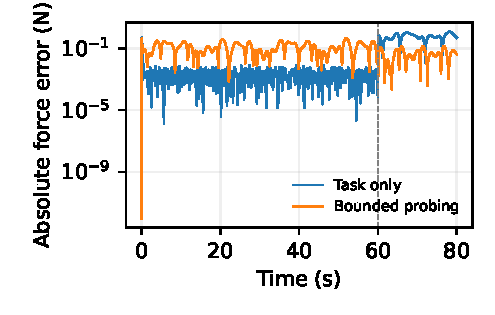
\includegraphics[width=.32\textwidth]{excitation_force.pdf}\hfill
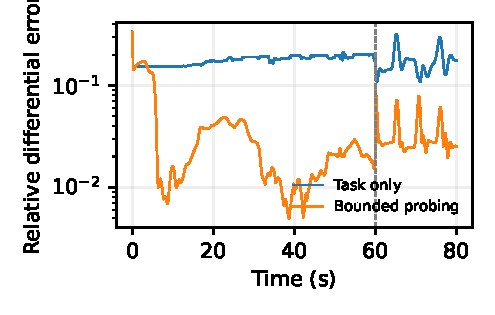
\includegraphics[width=.32\textwidth]{excitation_partial.pdf}\hfill
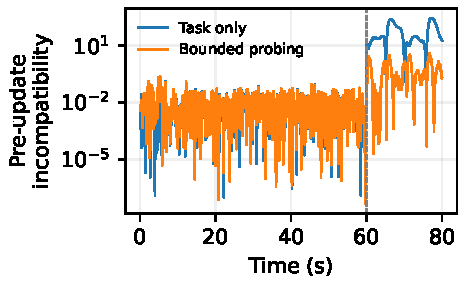
\includegraphics[width=.32\textwidth]{excitation_energy.pdf}\\
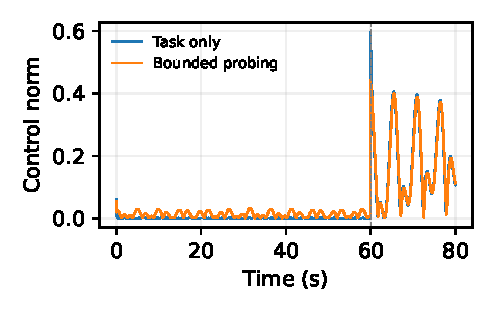
\includegraphics[width=.32\textwidth]{excitation_control.pdf}\hfill
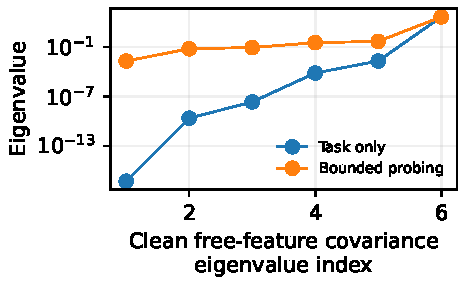
\includegraphics[width=.32\textwidth]{excitation_information.pdf}
\caption{Paired excitation. The trajectory panels show preselected seed 10.
Top row, left to right: force error,
relative differential error, and pre-update incompatibility. Bottom row:
applied command and the clean evaluator-only
information spectrum at the end of training, averaged over all ten seeds.
The vertical line marks
transfer to a new task with coefficients frozen. Clean information is not
provided to either learner.}
\label{fig:excitation}
\end{figure*}

The task-only controller maintains near-perfect regulation with negligible
control activity, and its incompatibility approaches the same-stream
true-model reference. Nevertheless its differential error remains substantial,
and its frozen model transfers poorly. The bounded probe incurs a training
tracking cost but yields substantially improved partial estimation and
transfer performance. These are illustrative outcomes for this specific
prescribed feature family and excitation signal; they do not imply a general
necessity or sufficiency theorem for task-specific learning.
